\section{FCFS}

El primer algoritmo evaluado fue FCFS (\textit{First Came First Save}). Se trata de la estrategia de scheduling m\'as sencilla. Te\'oricamente, est\'a representado por una cola que concede el recurso a cada tarea en un orden estricto de llegada. Cuando cada uno de los procesos pasa a estado READY, se agrega a una cola global. A medida que el proceso que se encuentra ejecutando termina, se selecciona al proceso que m\'as tiempo ha estado en esta cola.

Este algoritmo ya estaba implementado por la c\'atedra y se encuentra en el archivo \verb+sched_fcfs.cpp+. Para evaluarlo, el \textbf{ejercicio 1} solicitaba programar una tarea TaskConsola, que simulaba un proceso interactivo. La tarea recibe como par\'ametro:

\begin{enumerate}
	\item \textit{n}: que indica la cantidad de llamadas bloqueantes de la tarea.
	
	\item \textit{bmin}: la cota inferior de duraci\'on de cada llamada bloqueante
	
	\item \textit{bmax}: la cota superior de duraci\'on de cada llamada bloqueante.
\end{enumerate}

Se encuentra implementada como la funci\'on TaskConsola en el archivo \verb+tasks.cpp+.

La funci\'on deb\'ia realizar llamadas bloqueantes de duraci\'on aleatoria. Para simular ese comportamiento, se us\'o la funci\'on \textit{rand} que devuelve un n\'umero pseudoaleatorio entre 0 y \verb+MAX_RAND+\footnote{Se trata de un macro que depende de la implementaci\'on de la librer\'ia est\'andar de C. Se garantiza que es al menos 32767}. Para que la duraci\'on entrara en un rango, le sacamos el m\'odulo de a la diferencia entre \textit{bmax} y \textit{bmin} y le sumamos el valor \textit{bmin}:

\begin{verbatim}
    unsigned int bmax = params[2];	// la duracion maxima de la llamada bloqueante
    unsigned int bmin = params[1];  // la duracion minima de la llamada bloqueante
    unsigned int n = params[0];	// la cnatidad de llamadas bloqueantes
    for (unsigned int i = 0; i < n; i++) { // realizo n llamadas bloqueantes
        int duracion = rand()%(bmax - bmin) + bmin;	// número aleatorio 
        												//entre dos números
        uso_IO(pid, duracion); // realizo las llamadas bloqueantes
    }
\end{verbatim}

El \textbf{ejercicio 2} solicitaba realizar pruebas con lotes de tareas sobre el scheduler FCFS. Se deb\'ia realizar un lote de tres tareas usando el algoritmo FCFS para 1, 2 y 3 n\'ucleos:

\begin{verbatim}
TaskCPU 3
TaskConsola 3 5 10
TaskConsola 3 5 10
\end{verbatim}

Todas las tareas entran en estado READY en el instante 3 y las tares de consola realizan 3 llamadas bloqueantes de 5 a 10 ticks de reloj de duraci\'on.

Los resultados fueron los siguientes:

\begin{figure}[H]
\caption{1 TaskCPU y 2 TaskConsole con 1 core}
++----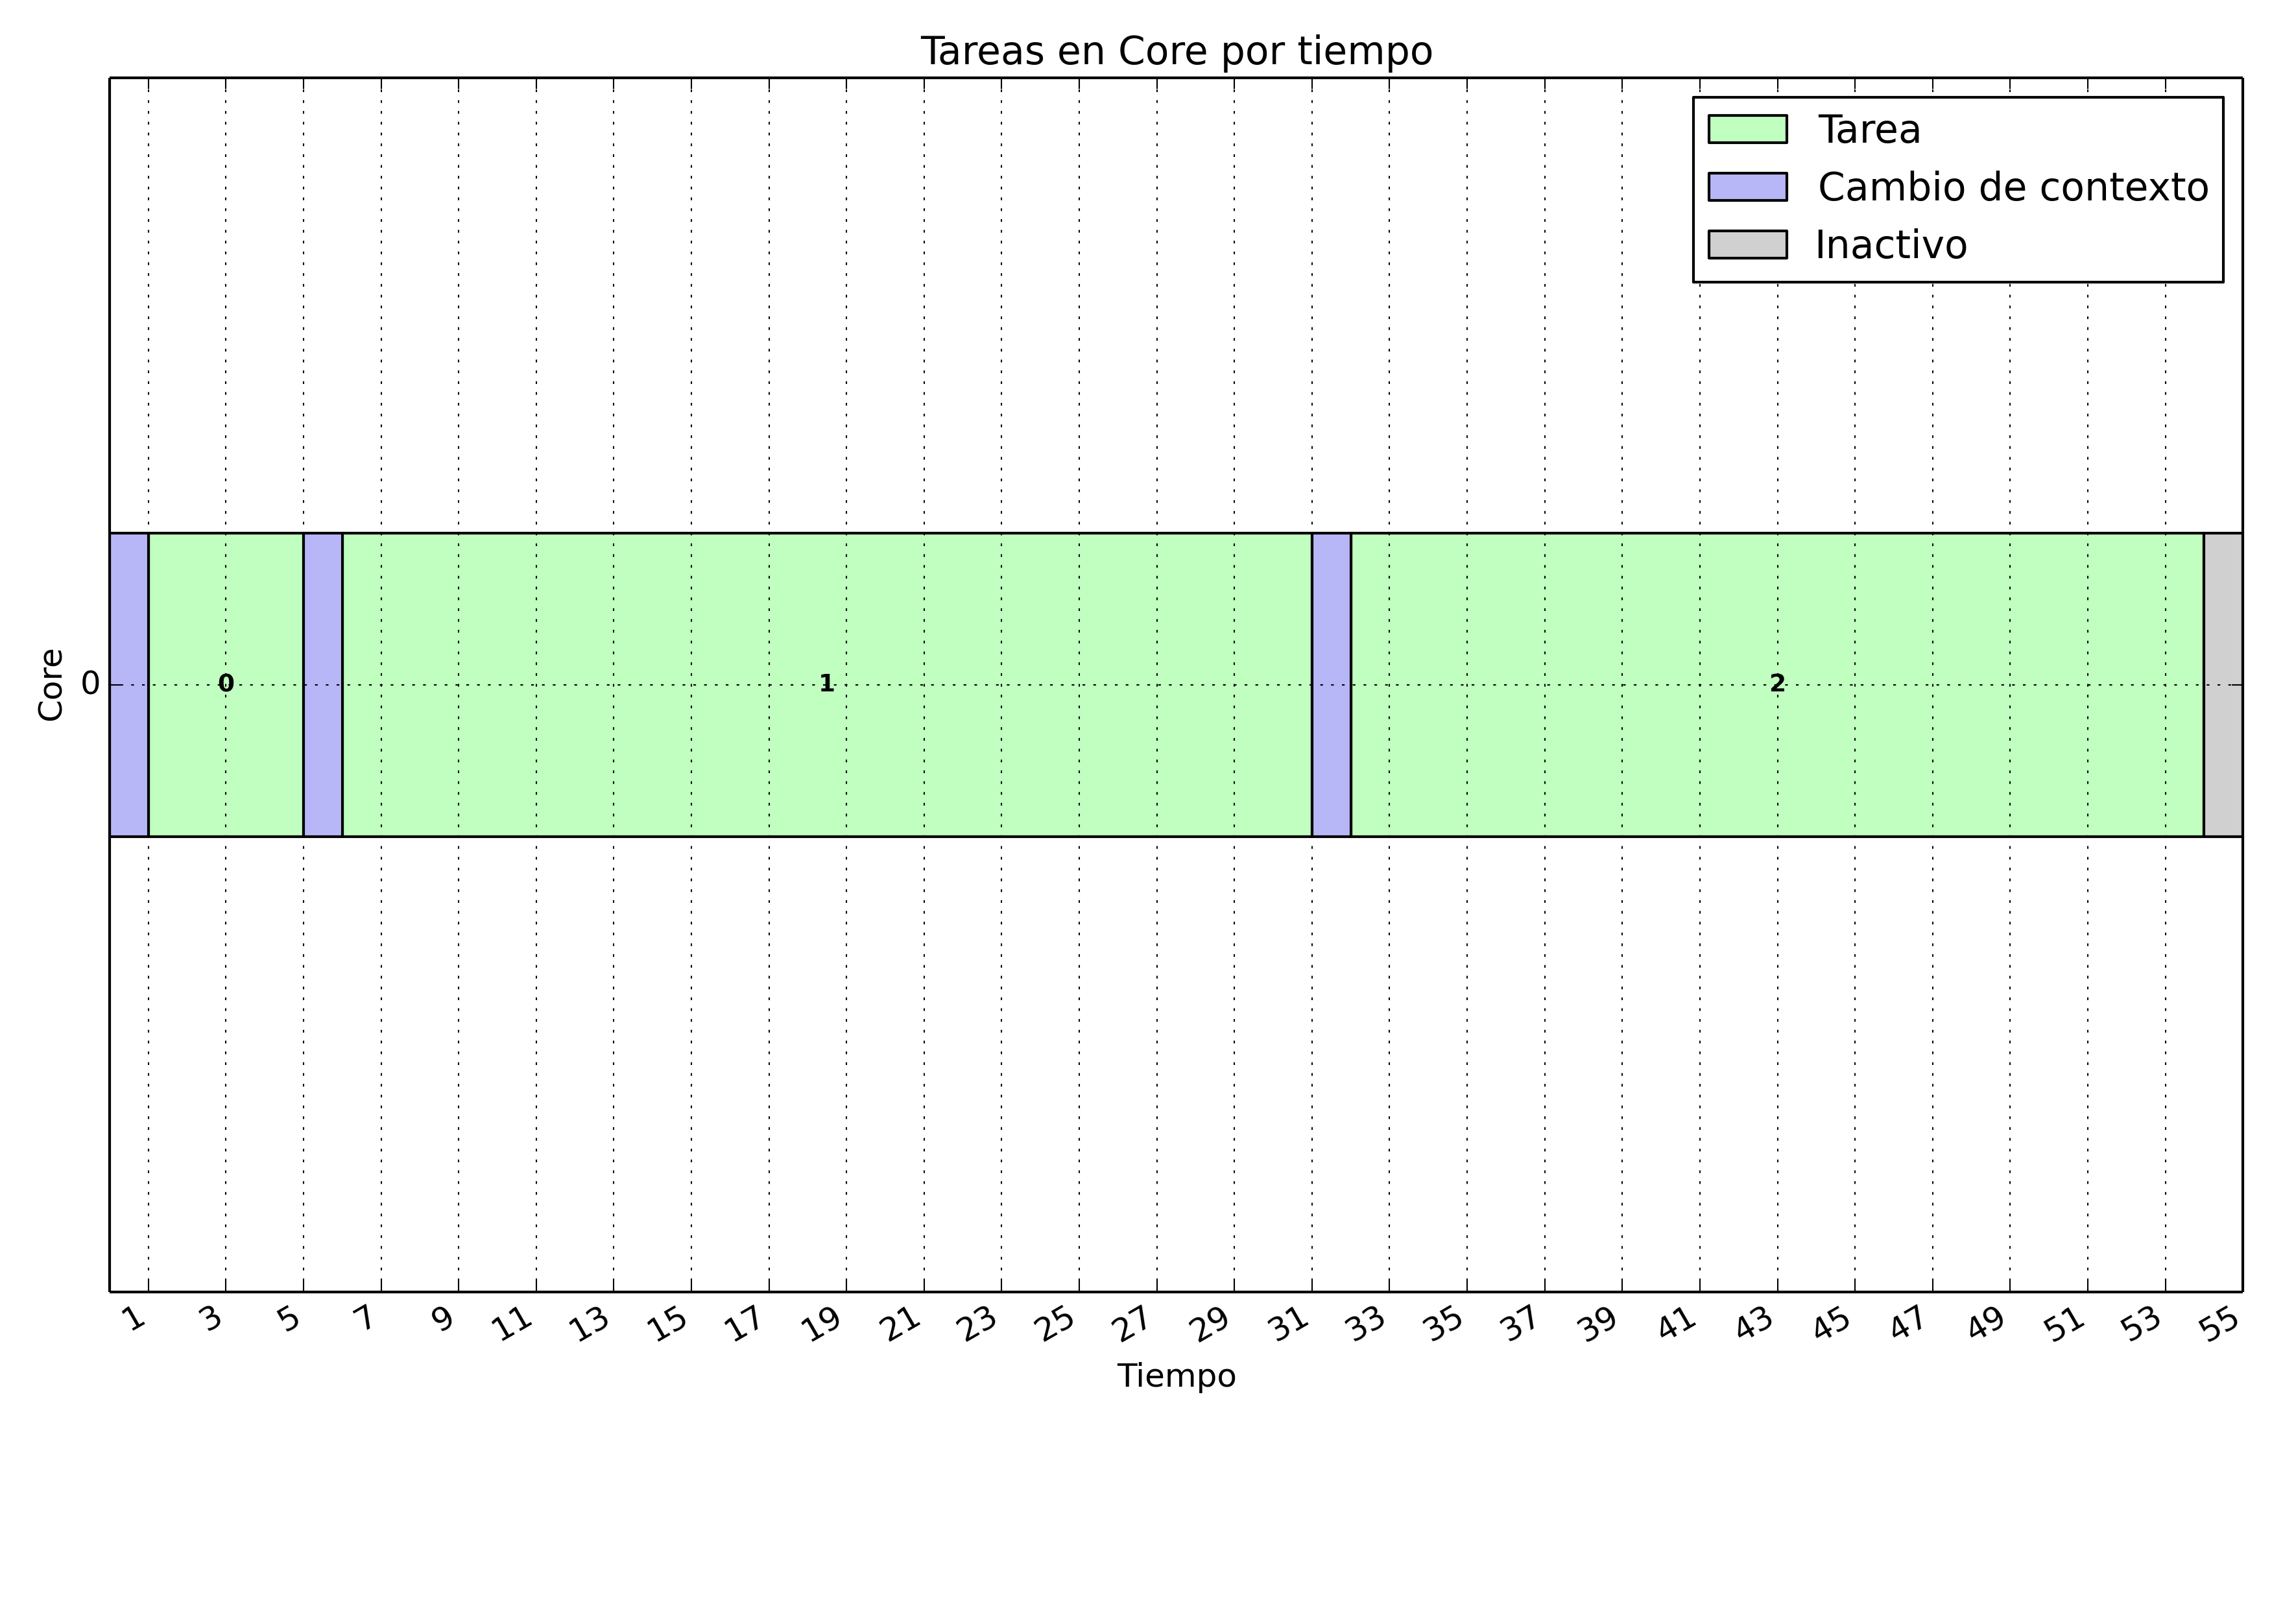
\includegraphics[width=\textwidth]{ejercicio_2_1}
\end{figure}

\begin{figure}[H]
\caption{1 TaskCPU y 2 TaskConsole con 2 cores}
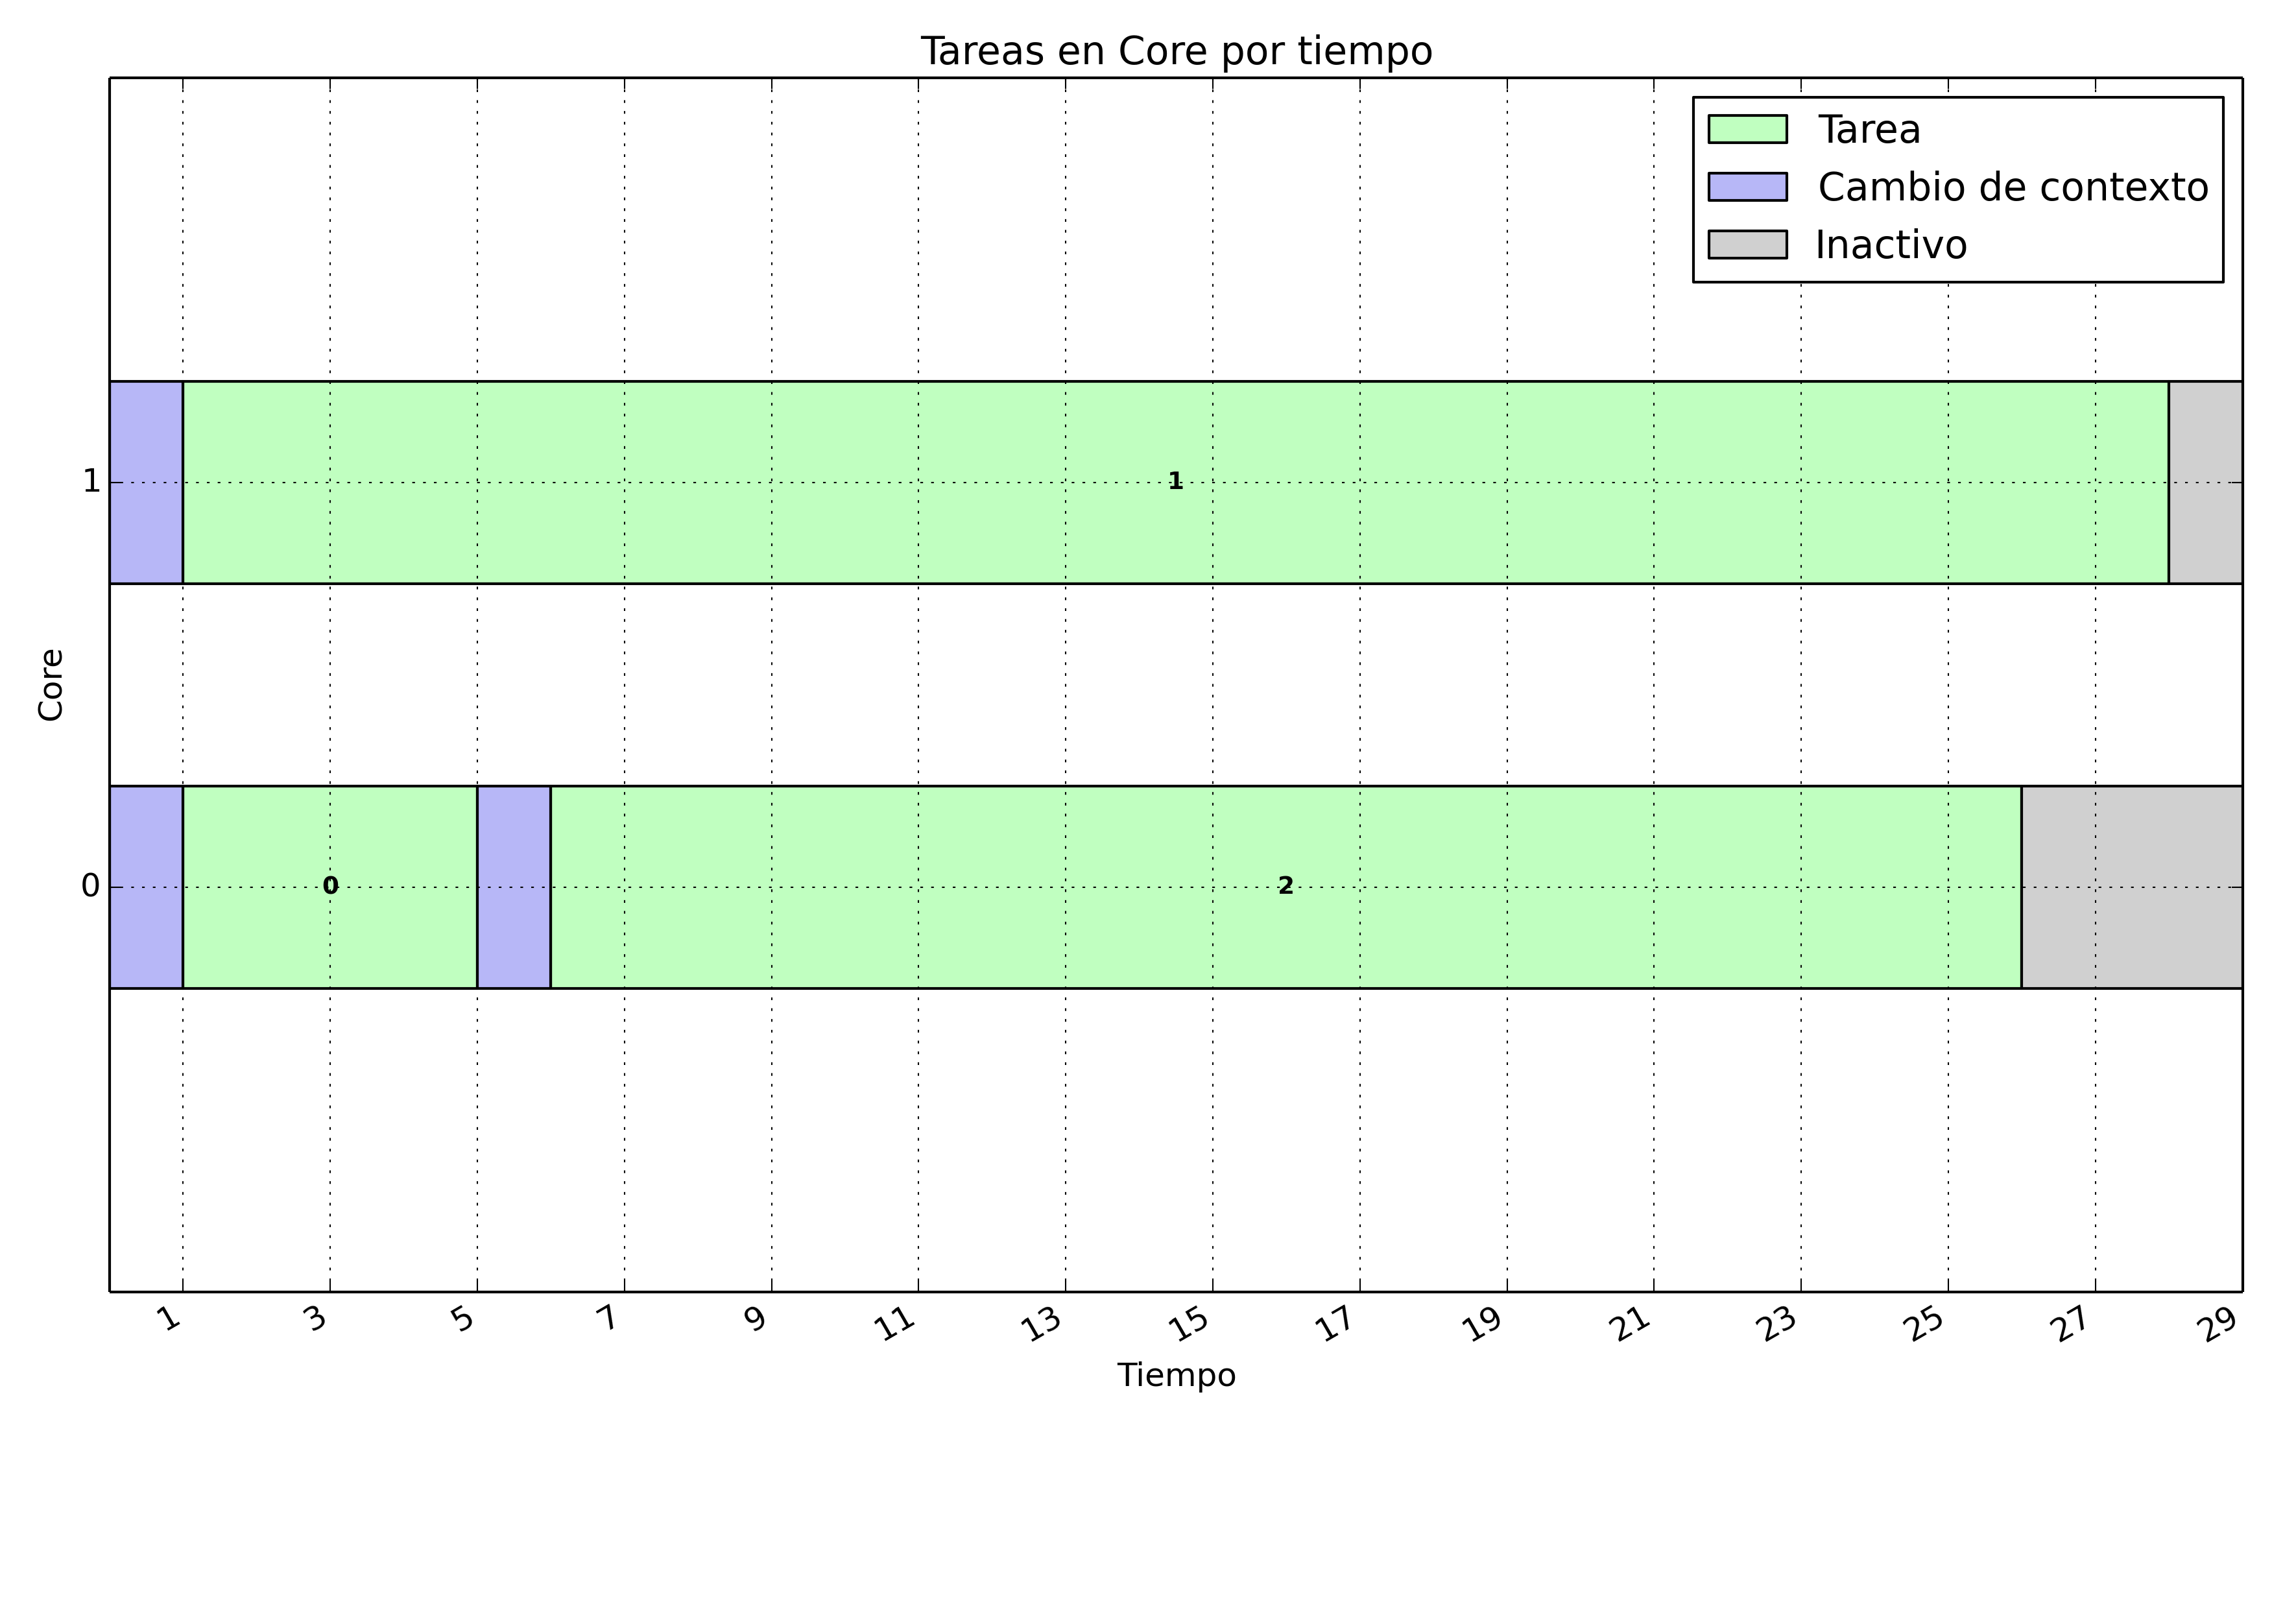
\includegraphics[width=\textwidth]{ejercicio_2_2}
\end{figure}

\begin{figure}[H]
\caption{1 TaskCPU y 2 TaskConsole con 3 cores}
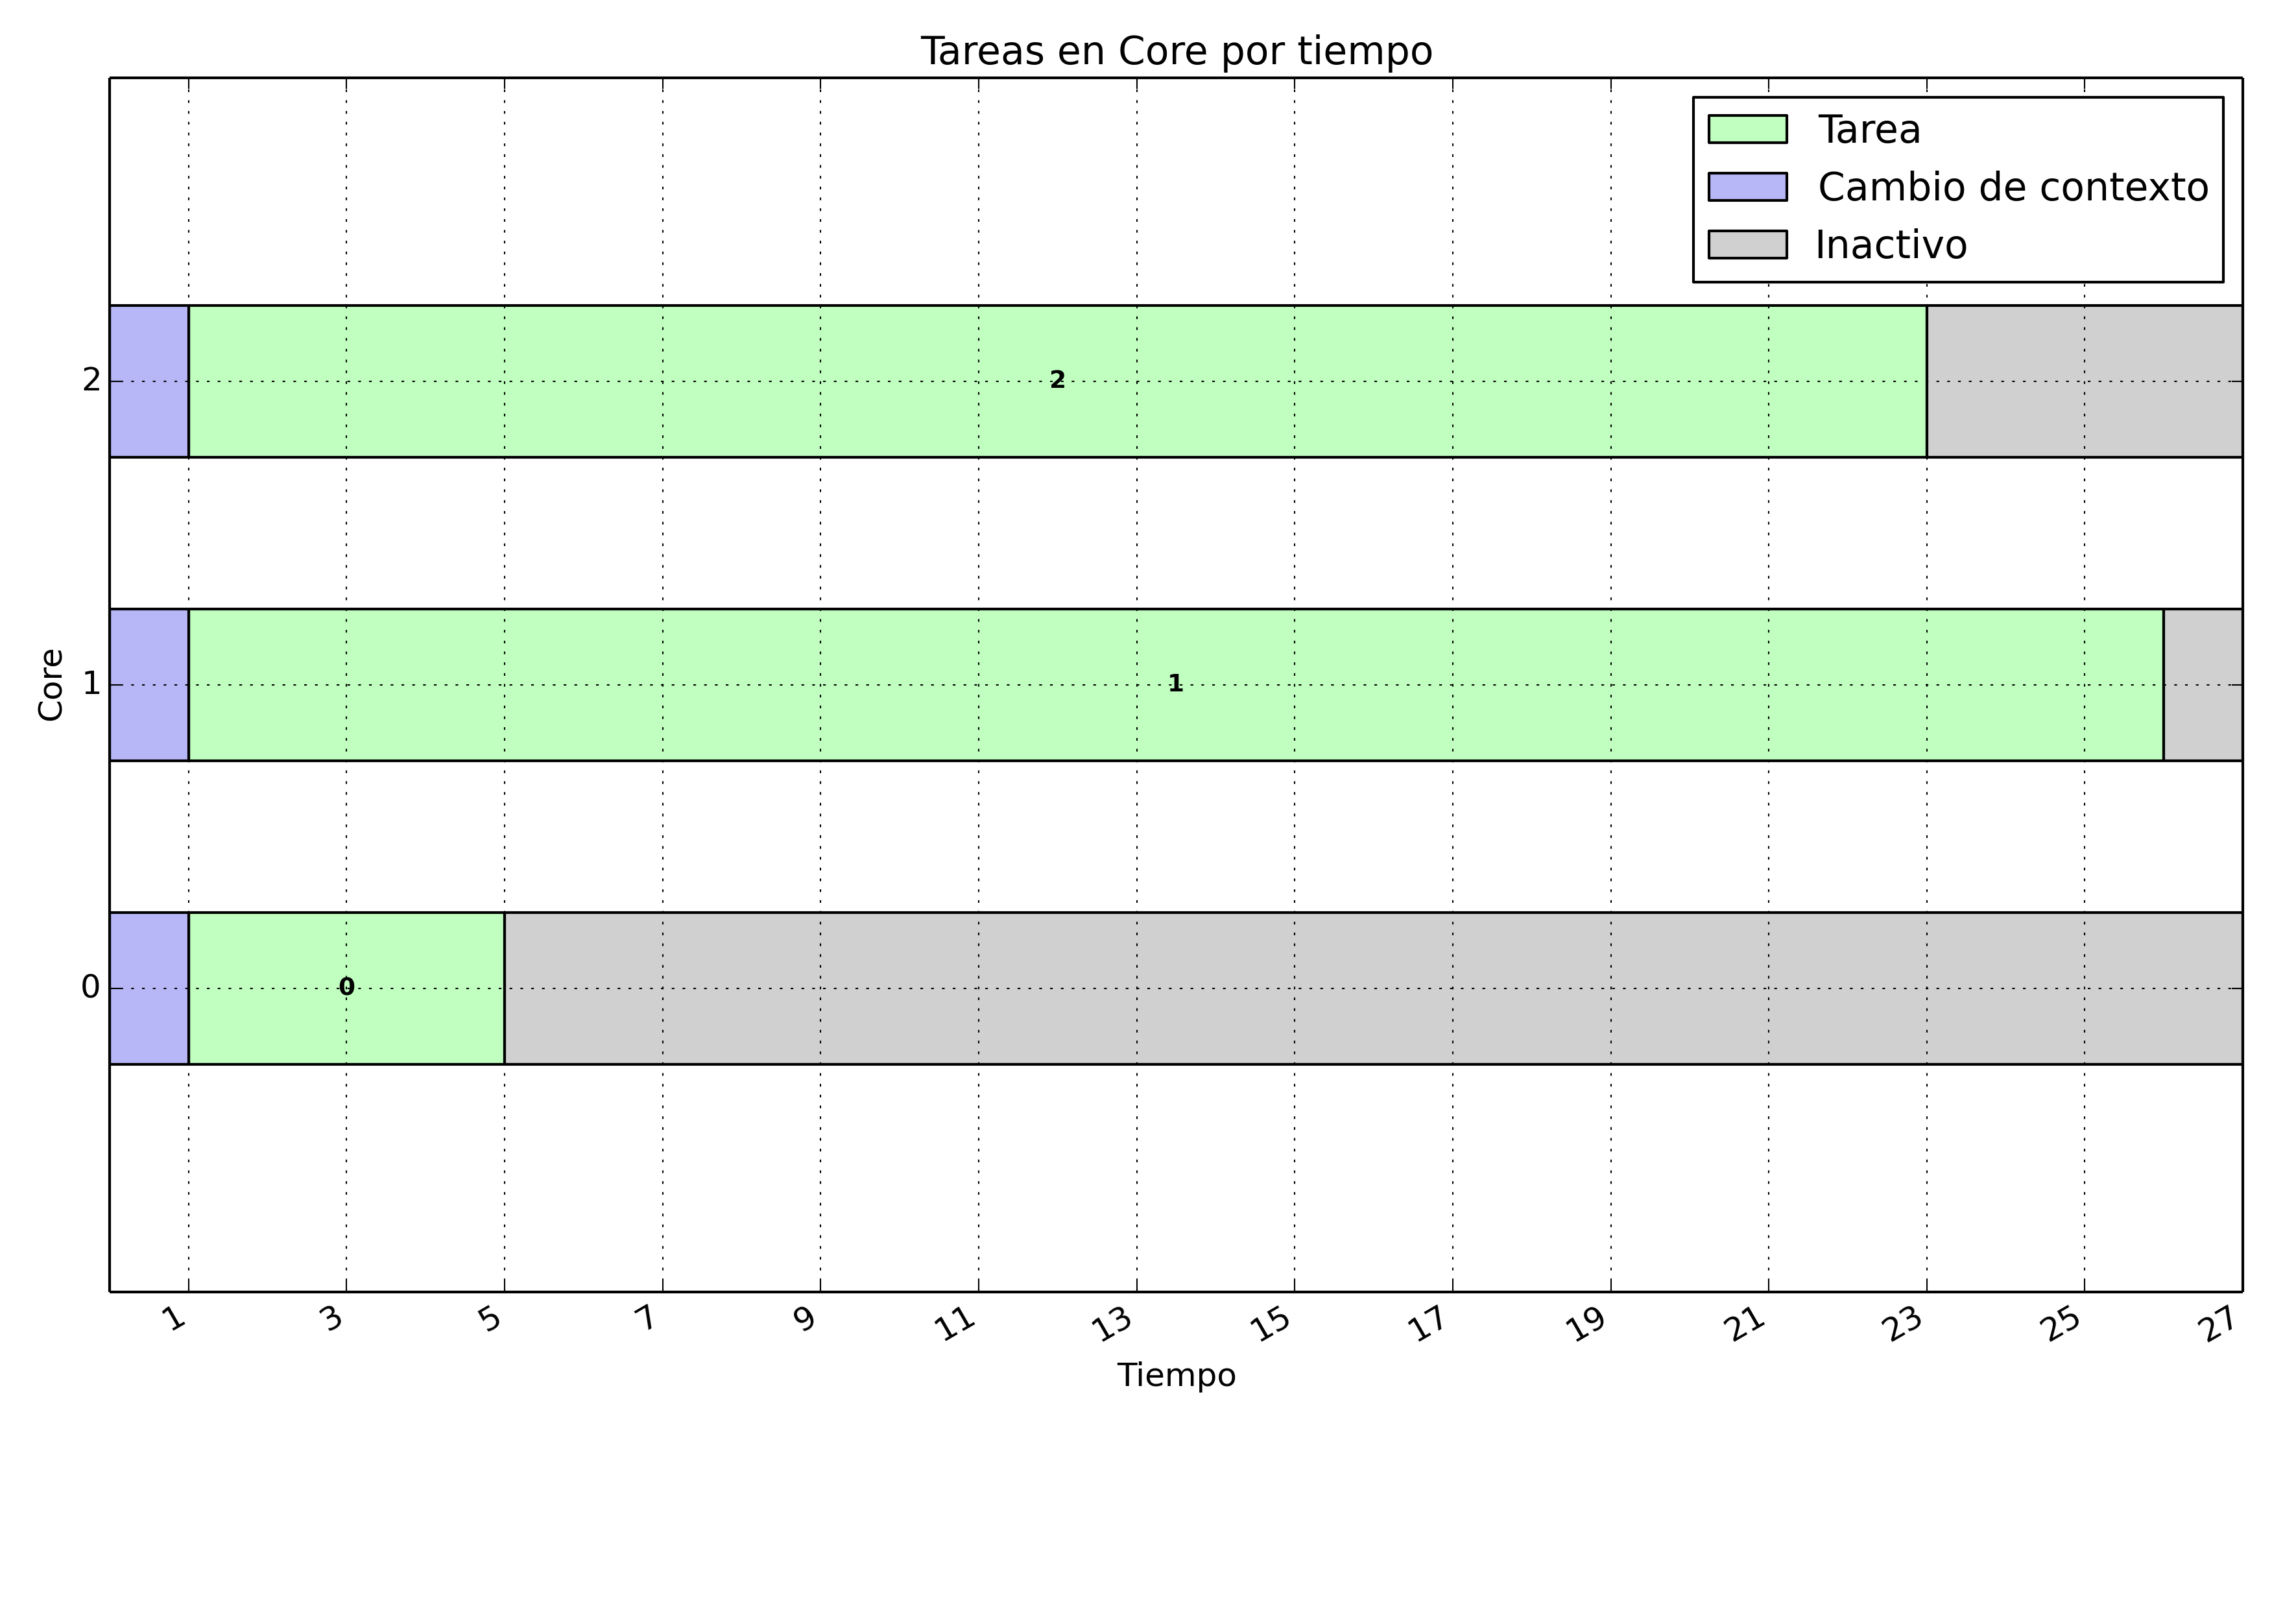
\includegraphics[width=\textwidth]{ejercicio_2_3}
\end{figure}

Se observa que no hay desalojo en esta estrategia de scheduling. De manera que cada vez que a una tarea se le concede el recurso CPU no lo libera hasta que termina su ejecuci\'on independientemente de los bloqueos que realice. Esto se implement\'o en el c\'odigo no realizando ninguna l\'ogica en la funci\'on que maneja el evento block. 

\begin{verbatim}
void SchedFCFS::unblock(int pid) {
    // Uy! unblock!... bueno, ya seguir'a en el próximo tick
}
\end{verbatim}

Observemos qu\'e sucede si las primera tareas que toman el procesador es la que que tarda m\'as en terminar. Usemos el siguiente lote, ejecutado en un core :

\begin{verbatim}
TaskConsola 3 5 10
TaskConsola 3 5 10
TaskCPU 1
\end{verbatim}

\begin{figure}[H]
\caption{1 TaskCPU de poca duraci\'on y 2 TaskConsole con 1 core}
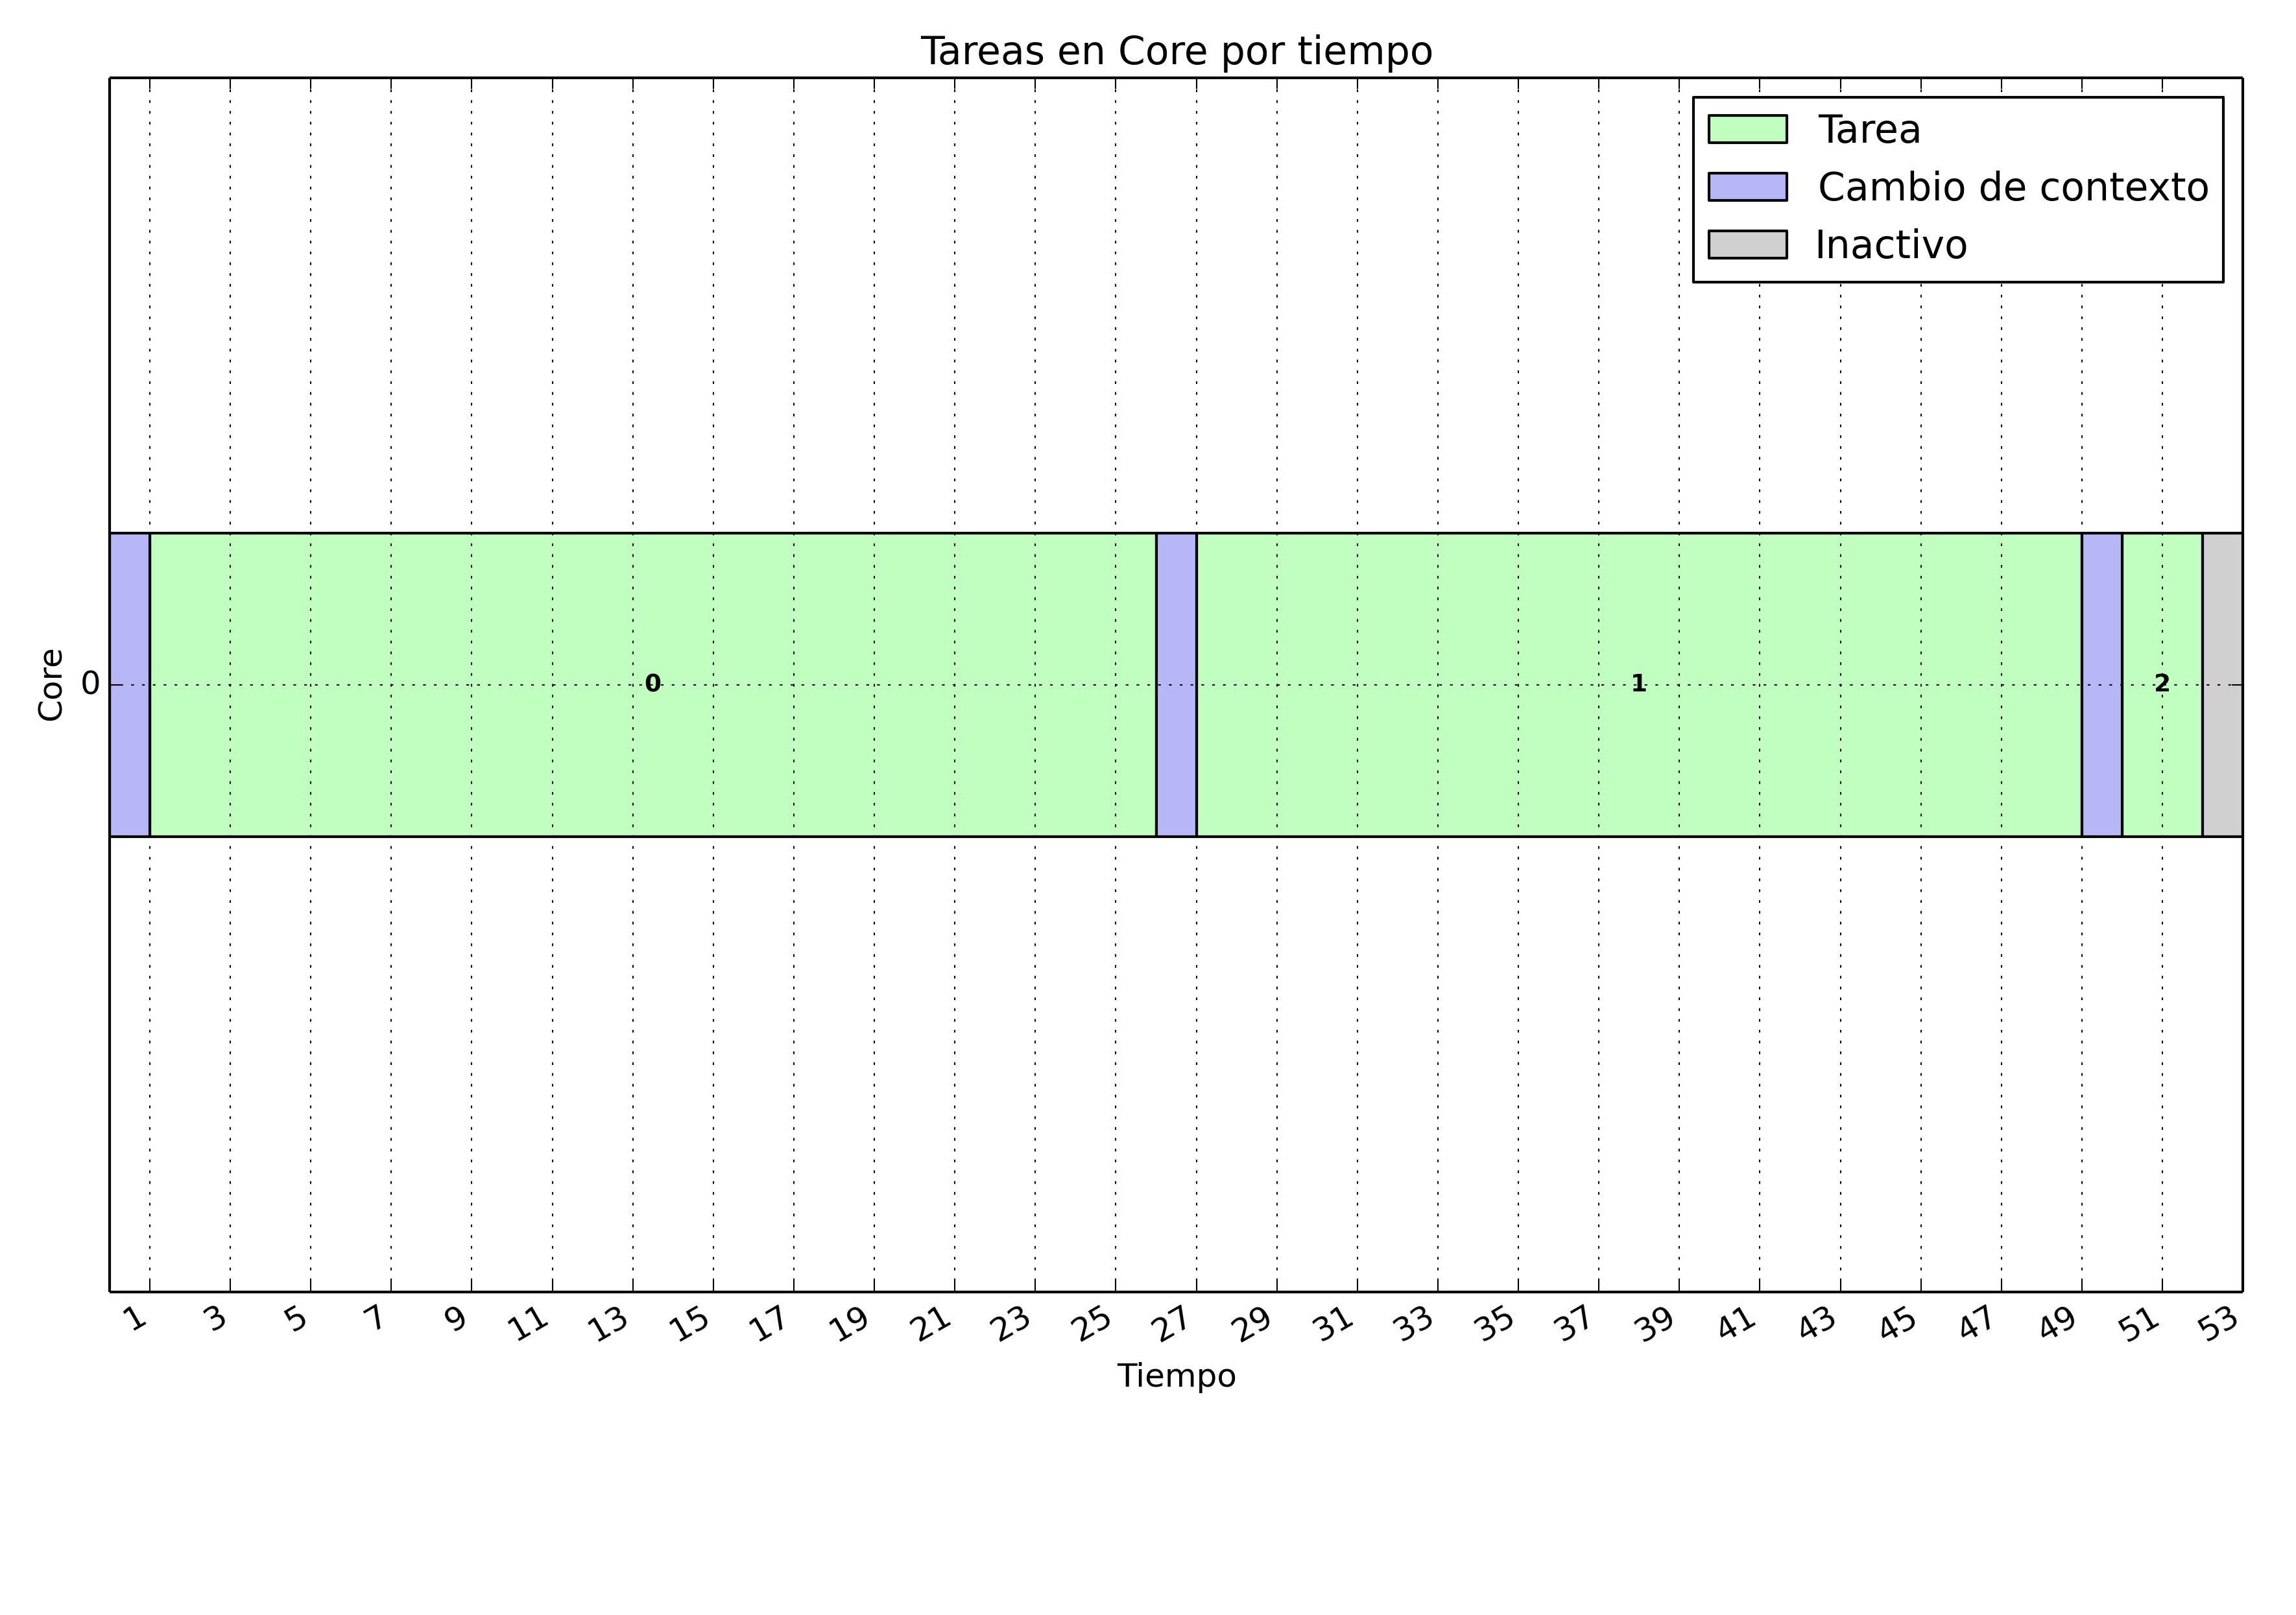
\includegraphics[width=\textwidth]{ejercicio_2_4}
\end{figure}

Como señalan varios autores \cite[p.~414]{stallings2008} \cite[p.~134]{tanenbaum2001}, este tipo de estrategias de scheduling funciona mejor para procesos cortos que para procesos de larga duraci\'on. Observamos en el lote anterior, que la tarea 3 tuvo un \textit{waiting time} de 49 ticks de reloj. Esto se aten\'ua en los lotes en los que se puede enviar la tarea a otro procesador. FCSF no parece muy atractivo para el modelo de \'unico core.